\documentclass[]{article}
\usepackage{lmodern}
\usepackage{amssymb,amsmath}
\usepackage{ifxetex,ifluatex}
\usepackage{fixltx2e} % provides \textsubscript
\ifnum 0\ifxetex 1\fi\ifluatex 1\fi=0 % if pdftex
  \usepackage[T1]{fontenc}
  \usepackage[utf8]{inputenc}
\else % if luatex or xelatex
  \ifxetex
    \usepackage{mathspec}
  \else
    \usepackage{fontspec}
  \fi
  \defaultfontfeatures{Ligatures=TeX,Scale=MatchLowercase}
\fi
% use upquote if available, for straight quotes in verbatim environments
\IfFileExists{upquote.sty}{\usepackage{upquote}}{}
% use microtype if available
\IfFileExists{microtype.sty}{%
\usepackage{microtype}
\UseMicrotypeSet[protrusion]{basicmath} % disable protrusion for tt fonts
}{}
\usepackage[margin=1in]{geometry}
\usepackage{hyperref}
\hypersetup{unicode=true,
            pdftitle={Urban\_mobility},
            pdfauthor={Ivana Kocanova},
            pdfborder={0 0 0},
            breaklinks=true}
\urlstyle{same}  % don't use monospace font for urls
\usepackage{color}
\usepackage{fancyvrb}
\newcommand{\VerbBar}{|}
\newcommand{\VERB}{\Verb[commandchars=\\\{\}]}
\DefineVerbatimEnvironment{Highlighting}{Verbatim}{commandchars=\\\{\}}
% Add ',fontsize=\small' for more characters per line
\usepackage{framed}
\definecolor{shadecolor}{RGB}{248,248,248}
\newenvironment{Shaded}{\begin{snugshade}}{\end{snugshade}}
\newcommand{\AlertTok}[1]{\textcolor[rgb]{0.94,0.16,0.16}{#1}}
\newcommand{\AnnotationTok}[1]{\textcolor[rgb]{0.56,0.35,0.01}{\textbf{\textit{#1}}}}
\newcommand{\AttributeTok}[1]{\textcolor[rgb]{0.77,0.63,0.00}{#1}}
\newcommand{\BaseNTok}[1]{\textcolor[rgb]{0.00,0.00,0.81}{#1}}
\newcommand{\BuiltInTok}[1]{#1}
\newcommand{\CharTok}[1]{\textcolor[rgb]{0.31,0.60,0.02}{#1}}
\newcommand{\CommentTok}[1]{\textcolor[rgb]{0.56,0.35,0.01}{\textit{#1}}}
\newcommand{\CommentVarTok}[1]{\textcolor[rgb]{0.56,0.35,0.01}{\textbf{\textit{#1}}}}
\newcommand{\ConstantTok}[1]{\textcolor[rgb]{0.00,0.00,0.00}{#1}}
\newcommand{\ControlFlowTok}[1]{\textcolor[rgb]{0.13,0.29,0.53}{\textbf{#1}}}
\newcommand{\DataTypeTok}[1]{\textcolor[rgb]{0.13,0.29,0.53}{#1}}
\newcommand{\DecValTok}[1]{\textcolor[rgb]{0.00,0.00,0.81}{#1}}
\newcommand{\DocumentationTok}[1]{\textcolor[rgb]{0.56,0.35,0.01}{\textbf{\textit{#1}}}}
\newcommand{\ErrorTok}[1]{\textcolor[rgb]{0.64,0.00,0.00}{\textbf{#1}}}
\newcommand{\ExtensionTok}[1]{#1}
\newcommand{\FloatTok}[1]{\textcolor[rgb]{0.00,0.00,0.81}{#1}}
\newcommand{\FunctionTok}[1]{\textcolor[rgb]{0.00,0.00,0.00}{#1}}
\newcommand{\ImportTok}[1]{#1}
\newcommand{\InformationTok}[1]{\textcolor[rgb]{0.56,0.35,0.01}{\textbf{\textit{#1}}}}
\newcommand{\KeywordTok}[1]{\textcolor[rgb]{0.13,0.29,0.53}{\textbf{#1}}}
\newcommand{\NormalTok}[1]{#1}
\newcommand{\OperatorTok}[1]{\textcolor[rgb]{0.81,0.36,0.00}{\textbf{#1}}}
\newcommand{\OtherTok}[1]{\textcolor[rgb]{0.56,0.35,0.01}{#1}}
\newcommand{\PreprocessorTok}[1]{\textcolor[rgb]{0.56,0.35,0.01}{\textit{#1}}}
\newcommand{\RegionMarkerTok}[1]{#1}
\newcommand{\SpecialCharTok}[1]{\textcolor[rgb]{0.00,0.00,0.00}{#1}}
\newcommand{\SpecialStringTok}[1]{\textcolor[rgb]{0.31,0.60,0.02}{#1}}
\newcommand{\StringTok}[1]{\textcolor[rgb]{0.31,0.60,0.02}{#1}}
\newcommand{\VariableTok}[1]{\textcolor[rgb]{0.00,0.00,0.00}{#1}}
\newcommand{\VerbatimStringTok}[1]{\textcolor[rgb]{0.31,0.60,0.02}{#1}}
\newcommand{\WarningTok}[1]{\textcolor[rgb]{0.56,0.35,0.01}{\textbf{\textit{#1}}}}
\usepackage{graphicx,grffile}
\makeatletter
\def\maxwidth{\ifdim\Gin@nat@width>\linewidth\linewidth\else\Gin@nat@width\fi}
\def\maxheight{\ifdim\Gin@nat@height>\textheight\textheight\else\Gin@nat@height\fi}
\makeatother
% Scale images if necessary, so that they will not overflow the page
% margins by default, and it is still possible to overwrite the defaults
% using explicit options in \includegraphics[width, height, ...]{}
\setkeys{Gin}{width=\maxwidth,height=\maxheight,keepaspectratio}
\IfFileExists{parskip.sty}{%
\usepackage{parskip}
}{% else
\setlength{\parindent}{0pt}
\setlength{\parskip}{6pt plus 2pt minus 1pt}
}
\setlength{\emergencystretch}{3em}  % prevent overfull lines
\providecommand{\tightlist}{%
  \setlength{\itemsep}{0pt}\setlength{\parskip}{0pt}}
\setcounter{secnumdepth}{0}
% Redefines (sub)paragraphs to behave more like sections
\ifx\paragraph\undefined\else
\let\oldparagraph\paragraph
\renewcommand{\paragraph}[1]{\oldparagraph{#1}\mbox{}}
\fi
\ifx\subparagraph\undefined\else
\let\oldsubparagraph\subparagraph
\renewcommand{\subparagraph}[1]{\oldsubparagraph{#1}\mbox{}}
\fi

%%% Use protect on footnotes to avoid problems with footnotes in titles
\let\rmarkdownfootnote\footnote%
\def\footnote{\protect\rmarkdownfootnote}

%%% Change title format to be more compact
\usepackage{titling}

% Create subtitle command for use in maketitle
\providecommand{\subtitle}[1]{
  \posttitle{
    \begin{center}\large#1\end{center}
    }
}

\setlength{\droptitle}{-2em}

  \title{Urban\_mobility}
    \pretitle{\vspace{\droptitle}\centering\huge}
  \posttitle{\par}
    \author{Ivana Kocanova}
    \preauthor{\centering\large\emph}
  \postauthor{\par}
      \predate{\centering\large\emph}
  \postdate{\par}
    \date{23/08/2019}


\begin{document}
\maketitle

To better understand urban life, this research aims to construct
networks utilizing travel-flow data. Using latest research of complex
networks, we plan to uncover inherent community structure within city of
Leeds. We believe these findings could be beneficial for urban planners,
infrastructure maintenance and epidemic outbreak management.

\hypertarget{exploring-origin-destionation-flows}{%
\subsubsection{Exploring Origin-Destionation
flows}\label{exploring-origin-destionation-flows}}

We begin by loading the Origin-destination flows and linking them with
spatial information loaded through shapefiles.

\begin{Shaded}
\begin{Highlighting}[]
\CommentTok{# Required packages}
\KeywordTok{library}\NormalTok{(sf)}
\end{Highlighting}
\end{Shaded}

\begin{verbatim}
## Linking to GEOS 3.6.1, GDAL 2.2.3, PROJ 4.9.3
\end{verbatim}

\begin{Shaded}
\begin{Highlighting}[]
\KeywordTok{library}\NormalTok{(stplanr)}
\end{Highlighting}
\end{Shaded}

\begin{verbatim}
## Registered S3 method overwritten by 'R.oo':
##   method        from       
##   throw.default R.methodsS3
\end{verbatim}

\begin{Shaded}
\begin{Highlighting}[]
\KeywordTok{library}\NormalTok{(leaflet)}
\KeywordTok{library}\NormalTok{(tmap)}
\KeywordTok{library}\NormalTok{(dplyr)}
\end{Highlighting}
\end{Shaded}

\begin{verbatim}
## 
## Attaching package: 'dplyr'
\end{verbatim}

\begin{verbatim}
## The following objects are masked from 'package:stats':
## 
##     filter, lag
\end{verbatim}

\begin{verbatim}
## The following objects are masked from 'package:base':
## 
##     intersect, setdiff, setequal, union
\end{verbatim}

\begin{Shaded}
\begin{Highlighting}[]
\KeywordTok{library}\NormalTok{(igraph)}
\end{Highlighting}
\end{Shaded}

\begin{verbatim}
## 
## Attaching package: 'igraph'
\end{verbatim}

\begin{verbatim}
## The following objects are masked from 'package:dplyr':
## 
##     as_data_frame, groups, union
\end{verbatim}

\begin{verbatim}
## The following objects are masked from 'package:stats':
## 
##     decompose, spectrum
\end{verbatim}

\begin{verbatim}
## The following object is masked from 'package:base':
## 
##     union
\end{verbatim}

\begin{Shaded}
\begin{Highlighting}[]
\KeywordTok{library}\NormalTok{(ggraph)}
\end{Highlighting}
\end{Shaded}

\begin{verbatim}
## Loading required package: ggplot2
\end{verbatim}

\begin{Shaded}
\begin{Highlighting}[]
\KeywordTok{tmap_mode}\NormalTok{(}\StringTok{"plot"}\NormalTok{)}
\end{Highlighting}
\end{Shaded}

\begin{verbatim}
## tmap mode set to plotting
\end{verbatim}

\begin{Shaded}
\begin{Highlighting}[]
\CommentTok{# Load the Origin-Destination (OD) flows}
\NormalTok{flows <-}\StringTok{ }\KeywordTok{read.csv}\NormalTok{(}\StringTok{"data}\CharTok{\textbackslash{}\textbackslash{}}\StringTok{2011_census_flows.csv"}\NormalTok{)}

\CommentTok{# Load Ward names lookup dataset}
\NormalTok{wards <-}
\StringTok{  }\KeywordTok{read.csv}\NormalTok{(}\StringTok{"data//Leeds_MSOA_Ward_LookUp.csv"}\NormalTok{)}

\CommentTok{# Read in shapefile containing MSOA boundaries}
\NormalTok{boundaries <-}
\StringTok{  }\NormalTok{sf}\OperatorTok{::}\KeywordTok{read_sf}\NormalTok{(}
    \StringTok{"data//boundaries//Middle_Layer_Super_Output_Areas_December_2011_Super_Generalised_Clipped_Boundaries_in_England_and_Wales.shp"}
\NormalTok{  )}

\CommentTok{# Filter boundaries for Leeds }
\NormalTok{leeds_boundaries <-}\StringTok{ }\NormalTok{boundaries }\OperatorTok
\StringTok{  }\KeywordTok{filter}\NormalTok{(stringr}\OperatorTok{::}\KeywordTok{str_detect}\NormalTok{(msoa11nm, }\StringTok{'Leeds'}\NormalTok{)) }\OperatorTok
\StringTok{  }\KeywordTok{st_transform}\NormalTok{(boundaries, }\DataTypeTok{crs =} \DecValTok{27700}\NormalTok{)}

\CommentTok{# Add ward names }
\NormalTok{leeds_OD_matrix <-}\StringTok{ }\NormalTok{flows }\OperatorTok\StringTok{ }
\StringTok{  }\KeywordTok{left_join}\NormalTok{(wards }\OperatorTok\StringTok{  }\KeywordTok{select}\NormalTok{(msoa, ward_name), }\DataTypeTok{by =} \KeywordTok{c}\NormalTok{(}\StringTok{"origin"}\NormalTok{ =}\StringTok{ "msoa"}\NormalTok{)) }\OperatorTok\StringTok{ }
\StringTok{  }\KeywordTok{rename}\NormalTok{(}\StringTok{"origin_ward"}\NormalTok{ =}\StringTok{ "ward_name"}\NormalTok{) }\OperatorTok\StringTok{ }
\StringTok{  }\KeywordTok{left_join}\NormalTok{(wards }\OperatorTok\StringTok{  }\KeywordTok{select}\NormalTok{(msoa, ward_name), }\DataTypeTok{by =} \KeywordTok{c}\NormalTok{(}\StringTok{"destination"}\NormalTok{ =}\StringTok{ "msoa"}\NormalTok{)) }\OperatorTok\StringTok{ }
\StringTok{  }\KeywordTok{rename}\NormalTok{(}\StringTok{"destination_ward"}\NormalTok{ =}\StringTok{ "ward_name"}\NormalTok{)}

\CommentTok{# Add the geometry information for MSOA's}
\NormalTok{leeds_OD_matrix <-}\StringTok{ }\NormalTok{leeds_OD_matrix }\OperatorTok
\StringTok{  }\KeywordTok{left_join}\NormalTok{(leeds_boundaries }\OperatorTok\StringTok{ }\KeywordTok{select}\NormalTok{(msoa11cd, geometry),}
            \DataTypeTok{by =} \KeywordTok{c}\NormalTok{(}\StringTok{"origin"}\NormalTok{ =}\StringTok{ "msoa11cd"}\NormalTok{)) }\OperatorTok
\StringTok{  }\KeywordTok{rename}\NormalTok{(}\StringTok{"geometry_origin"}\NormalTok{ =}\StringTok{ "geometry"}\NormalTok{) }\OperatorTok\StringTok{  }
\StringTok{  }\KeywordTok{left_join}\NormalTok{(leeds_boundaries }\OperatorTok\StringTok{ }\KeywordTok{select}\NormalTok{(msoa11cd, geometry),}
          \DataTypeTok{by =} \KeywordTok{c}\NormalTok{(}\StringTok{"destination"}\NormalTok{ =}\StringTok{ "msoa11cd"}\NormalTok{)) }\OperatorTok
\StringTok{  }\KeywordTok{rename}\NormalTok{(}\StringTok{"geometry_destination"}\NormalTok{ =}\StringTok{ "geometry"}\NormalTok{)}

\KeywordTok{rm}\NormalTok{(leeds_boundaries)}
\end{Highlighting}
\end{Shaded}

\hypertarget{which-areas-are-losinggaining-population-throughout-the-day}{%
\subsubsection{Which areas are losing/gaining population throughout the
day}\label{which-areas-are-losinggaining-population-throughout-the-day}}

The following section examines which areas of Leeds experience
population inflows or outflows. Having such insight can be valuable for
infrastructure planners or city councils to effectively distribute
resources.

\begin{Shaded}
\begin{Highlighting}[]
\CommentTok{# Table of the most frequent origin wards}
\NormalTok{o_table <-}\StringTok{ }\NormalTok{leeds_OD_matrix  }\OperatorTok
\StringTok{  }\KeywordTok{group_by}\NormalTok{(origin_ward) }\OperatorTok
\StringTok{  }\KeywordTok{summarize}\NormalTok{(}\DataTypeTok{o_count =} \KeywordTok{n}\NormalTok{()) }\OperatorTok
\StringTok{  }\KeywordTok{arrange}\NormalTok{(}\KeywordTok{desc}\NormalTok{(o_count))}

\CommentTok{# Table of the most frequent destination wards}
\NormalTok{d_table <-}\StringTok{ }\NormalTok{leeds_OD_matrix }\OperatorTok
\StringTok{  }\KeywordTok{group_by}\NormalTok{(destination_ward) }\OperatorTok
\StringTok{  }\KeywordTok{summarize}\NormalTok{(}\DataTypeTok{d_count =} \KeywordTok{n}\NormalTok{()) }\OperatorTok
\StringTok{  }\KeywordTok{arrange}\NormalTok{(}\KeywordTok{desc}\NormalTok{(d_count))}

\CommentTok{# Create a table which deducts the count of origins from destinations }
\NormalTok{final_table <-}\StringTok{ }\NormalTok{o_table }\OperatorTok\StringTok{ }\KeywordTok{left_join}\NormalTok{(d_table, }\DataTypeTok{by =} \KeywordTok{c}\NormalTok{(}\StringTok{"origin_ward"}\NormalTok{ =}\StringTok{ "destination_ward"}\NormalTok{))}
\NormalTok{final_table}\OperatorTok{$}\NormalTok{inflows_count <-}\StringTok{ }\NormalTok{final_table}\OperatorTok{$}\NormalTok{d_count }\OperatorTok{-}\StringTok{ }\NormalTok{final_table}\OperatorTok{$}\NormalTok{o_count }

\CommentTok{# Display the table of inflows }
\NormalTok{final_table }\OperatorTok\StringTok{ }
\StringTok{  }\KeywordTok{select}\NormalTok{(origin_ward,inflows_count) }\OperatorTok\StringTok{ }
\StringTok{  }\KeywordTok{arrange}\NormalTok{(}\KeywordTok{desc}\NormalTok{(inflows_count))}
\end{Highlighting}
\end{Shaded}

\begin{verbatim}
## # A tibble: 33 x 2
##    origin_ward                   inflows_count
##    <fct>                                 <int>
##  1 Burmantofts and Richmond Hill            41
##  2 City and Hunslet                         37
##  3 Morley South                             35
##  4 Beeston and Holbeck                      28
##  5 Hyde Park and Woodhouse                  25
##  6 Morley North                             20
##  7 Armley                                   19
##  8 Calverley and Farsley                    16
##  9 Killingbeck and Seacroft                 15
## 10 Farnley and Wortley                      14
## # ... with 23 more rows
\end{verbatim}

The table above shows that the Burmantofts and Richmond Hill had 41 more
recorded incoming flows than outflows. The areas with the highest
outflows were Wetherby, Kippax and Methley, and Ardsley and Robin Hood.

\begin{Shaded}
\begin{Highlighting}[]
\CommentTok{# Join inflows dataframe with wards }
\NormalTok{wards <-}\StringTok{ }\NormalTok{wards }\OperatorTok\StringTok{ }\KeywordTok{left_join}\NormalTok{(final_table, }\DataTypeTok{by =} \KeywordTok{c}\NormalTok{ (}\StringTok{"ward_name"}\NormalTok{ =}\StringTok{ "origin_ward"}\NormalTok{))}

\CommentTok{# Add spatial information about the wards}
\NormalTok{wards <-}\StringTok{ }\NormalTok{wards }\OperatorTok\StringTok{ }\KeywordTok{left_join}\NormalTok{(boundaries }\OperatorTok\StringTok{ }\KeywordTok{select}\NormalTok{(msoa11cd, geometry), }\DataTypeTok{by =} \KeywordTok{c}\NormalTok{(}\StringTok{"msoa"}\NormalTok{ =}\StringTok{ "msoa11cd"}\NormalTok{))}
\NormalTok{wards <-}\StringTok{ }\NormalTok{wards }\OperatorTok\StringTok{ }\KeywordTok{st_sf}\NormalTok{(}\DataTypeTok{sf_column_name =} \StringTok{"geometry"}\NormalTok{)}

\CommentTok{# Map of the inflows counts}
\KeywordTok{tm_shape}\NormalTok{(wards) }\OperatorTok{+}
\StringTok{  }\KeywordTok{tm_fill}\NormalTok{(}\DataTypeTok{col =} \StringTok{"inflows_count"}\NormalTok{, }\DataTypeTok{style =} \StringTok{"jenks"}\NormalTok{, }\DataTypeTok{midpoint =} \OtherTok{NA}\NormalTok{, }\DataTypeTok{alpha =} \FloatTok{0.7}\NormalTok{, }\DataTypeTok{title =} \StringTok{"Inflows count"}\NormalTok{)}\OperatorTok{+}
\StringTok{  }\KeywordTok{tm_borders}\NormalTok{() }\OperatorTok{+}\StringTok{ }
\StringTok{  }\KeywordTok{tm_basemap}\NormalTok{(}\DataTypeTok{server =} \StringTok{"OpenStreetMap.BlackAndWhite"}\NormalTok{)}
\end{Highlighting}
\end{Shaded}

\includegraphics{Markdown_analysis_files/figure-latex/unnamed-chunk-3-1.pdf}

The code above sums previously obtained table into heatmap highlighting
how different areas of Leeds are affected by urban mobility. It can be
observed that most inflows are consolidated around the centre and
highest outflows are within Wetherby and south-east parts of the Leeds.

\hypertarget{estimating-travel-routes-from-od-flows}{%
\subsubsection{Estimating travel routes from OD
flows}\label{estimating-travel-routes-from-od-flows}}

Knowing where a journey began and ended we can estimate the most likely
route taken. For example, a journey from Wetherby to Otley depicted as a
straight line can be transformed into a traffic route as seen in the
picture below.

\begin{figure}
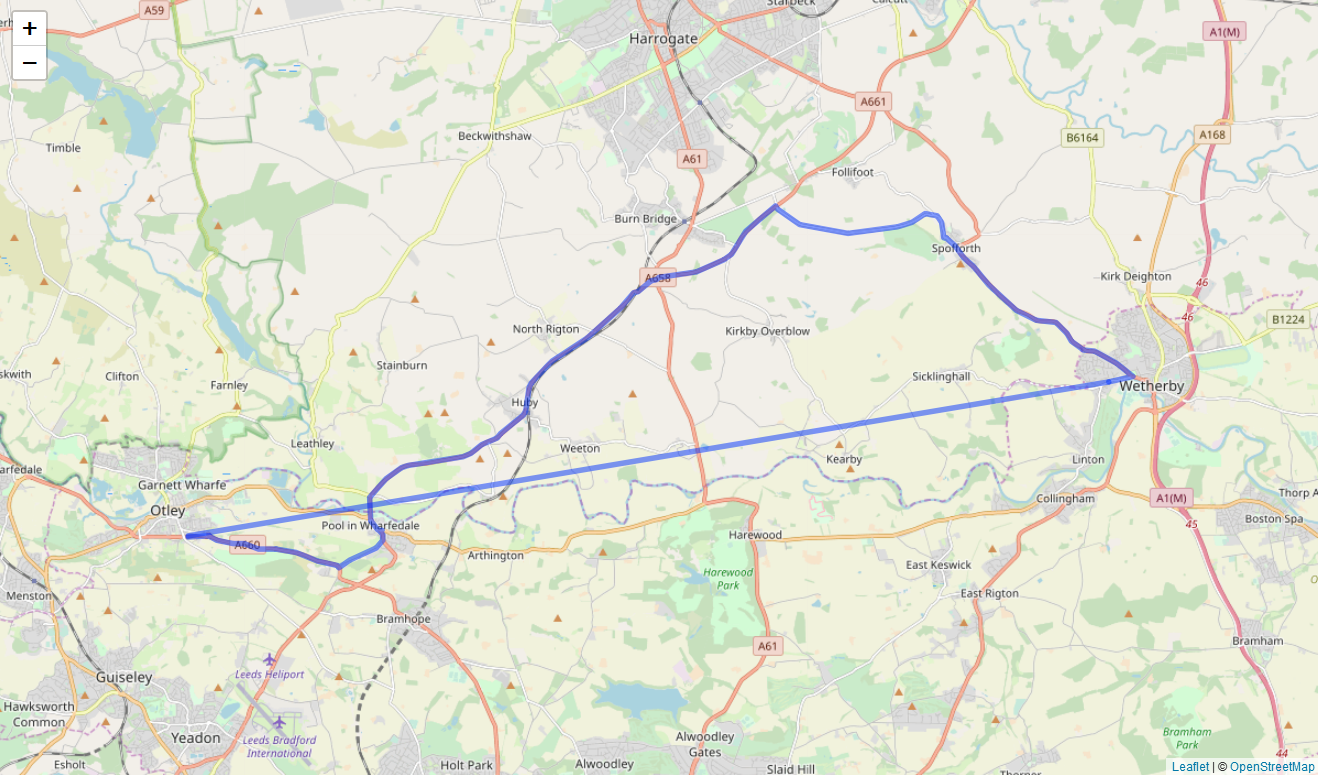
\includegraphics[width=1\linewidth]{maps\Example_line2route} \caption{Estimation of route taken between Wetherby and Otley}\label{fig:pressure}
\end{figure}

Having calculated the routes with OSRM, the route network can be then
visualized to show where the routes overlap each other. The darker
colour shows a higher frequency of individuals movement and indicates
places of possible traffic congestion.


\end{document}
